\documentclass[a4paper]{scrartcl}
\usepackage[utf8]{inputenc}
\usepackage[english]{babel}
\usepackage{graphicx}
\usepackage{lastpage}
\usepackage{pgf}
\usepackage{wrapfig}
\usepackage{fancyvrb}
\usepackage{fancyhdr}
\usepackage{hyperref}
\pagestyle{fancy}

\catcode`\_=\active
\protected\def_#1_{\textit{#1}}

% Create header and footer
\headheight 27pt
\pagestyle{fancyplain}
\lhead{\footnotesize{Distributed Systems - Advanced, ID2203}}
\chead{\footnotesize{Project}}
\rhead{}
\lfoot{}
\cfoot{\thepage}
\rfoot{}

% Create title page
\title{Distributed Key-Value Store}
\subtitle{Distributed Systems - Advanced, ID2203}
\author{Bernardo Gonzalez Riede \& Vinit Kumar Verma}
\date{\today}

\begin{document}

\maketitle

%Introduction
\section{Introduction}

\subsection{Goals}
The overall goal is to have a distributed, partitioned and in-memory key-value store. 
While not explicitly mentioned, the abstractions used throughout the course and the book are fundamental for planning and reasoning about the system development. Imbuing them and relying on underneath abstractions might reduce complexity considerably while working on a certain module/layer. 

\subsection{Requirements}
The following points had to be covered:
\begin{itemize}
\item Linearizable operation semantics
\item Development of test scenarios
\item _GET_, _PUT_ and _CAS_ operations
\end{itemize}

%Design choices
\section{Reasoning \& Motivation}

\subsection{Distributed system model assumption}

The model used is a combination of fail-silent and fail-noisy. On the small scale, i.e. in a replication group, the model is fail-silent while using a _Ballot Leader Election_. Fail-noisy is used on every node to have a global overview of suspected nodes.
The following sections will motivate the decision made.

\subsubsection{Process/crash abstraction}
Byzantine failures won’t be covered. While a reality, it introduces a significant amount of complexity. The probability of a malicious failure during the development is low enough to be negligible. Arbitrary faults in the form of corrupted messages will be prevented by using TCP/IP. Moreover, being a memory key value store one could argue about the usage of ECC buffered RAM which corrects corrupt memory, which itself is already an unlikely one-time failure.
If a node crashes, it won’t be restarted itself which makes omissions the only reason for using the crash-recovery model. Omissions may incur in the following way:

\begin{itemize}
\item A node is overloaded
\item A message is lost in transit
\item Network partition
\end{itemize}

A node overload can be prevented by vertical scaling while the perfect link abstraction assures exactly-once delivery.
For this project it’s feasible to assume that a high amount of crashes is unlikely, meaning a majority of correct nodes exists. Therefore the crash-stop model will be used.


\subsubsection{Communication assumptions}
Being the abstraction mostly used during the course and guaranteeing exactly-once delivery, perfect links will be used for communication.

\subsubsection{Timing assumptions}
Running the nodes on the same machine can allow for a synchronous system, although a growing key value store might pose a problem. While it might be possible to use this model in the real world, accounting for uncertainty has to be included and so a partially synchronous system is a better fit.

\subsection{Design choices}


\subsubsection{Bootstrapping}
Bootstrapping is the only weakness of the system.
During bootstrapping the bootstrap servers poses a single point of failure.
It reads the replication degree and the amount of partions wanted from a configuration file and waits until enough nodes have checked in to be able to form the distibuted \& partitioned KV-store.
It sends the generated lookup table to all nodes.

Each node then extracts the list of nodes of its own partitions to start the BLE for the partition.
Moreover, Ev.P is used to monitor all nodes in the system as to only provide a newly connected client only with a not suspected node as entry point

\subsubsection{Partitioning}
Partitioning is done automatically through the bootstrapping node which divides the total number space an _integer_ can have to create even partitions. 
This decision is the result of the provided code base which includes a _String.toHash()_ method returning an _integer_.

\subsubsection{Replication}
A shared memory abstraction is too weak to provide a compare and swap operation, therefore motivating the need of implementing a replicated state machine.
This was done using the _SequencePaxos_ algorithm from the course.

\subsubsection{Resilience}
The planned resilience is f=2 and to have replication groups for every partition of 5 nodes, thus having always a correct quorum. 3 is normally a good value and maybe the value of f will be changed to 1 to be able to reduce the quorums to 3. This depends on the load each node places on the development machines during testing. 

\subsubsection{Client}
The client only needs to know one correct process to be able to use the service.
It connects to one server, which in turn will return the address of a random node from the list of not suspected servers.
From there on he will use that server as entry point  





%Implementation
\section{Implementation}

\subsection{Codebase}
The scala codebase was used as a head start for the implementation.
Figure \ref{fig:initial} shows the component diagram of the provided scala code base. 

\begin{figure}[h!]
  \begin{center}
    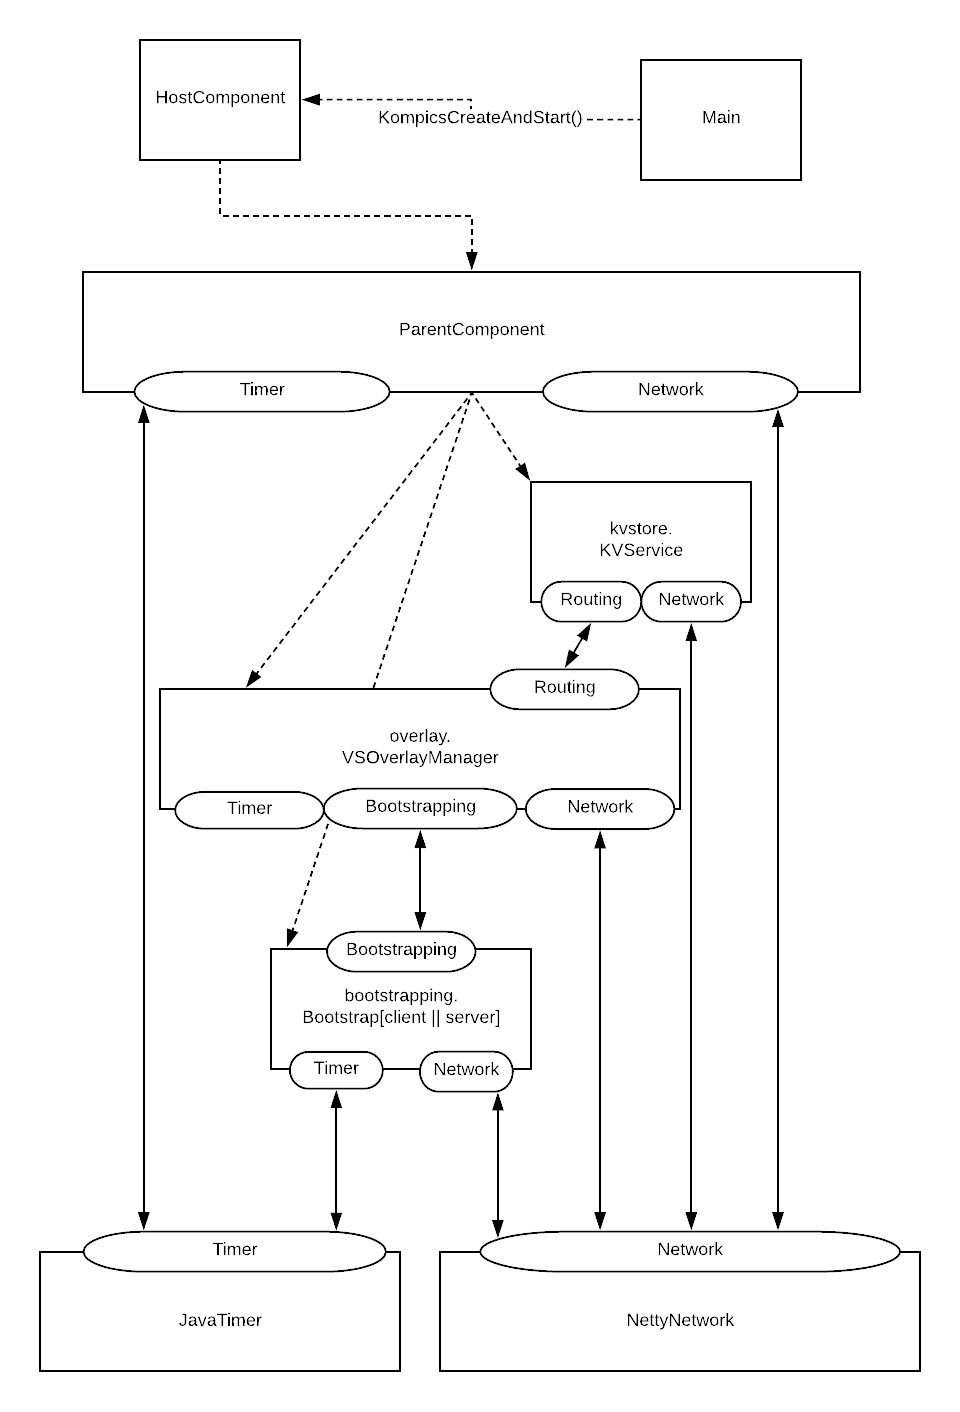
\includegraphics[scale=0.4]{Initial.png}
    \caption{Component Hierarchy of the code template}
    \label{fig:initial}
  \end{center}
\end{figure}

\subsection{Added code}
Figure \ref{fig:modified} shows only the added components and affected components from the template except _Timer_ and _Network_ which should be clear.
Furthermore the diagram shows the component using the network component although the code from the exercises rely on a _PerfectLink_ in the code. 
Being only a wrapper  for the network component the diagram shows no diferrence to the real world behaviour.
This is thanks to the underlying usage of TCP which provides session based FIFO perfect links.

\begin{figure}[h!]
  \begin{center}
    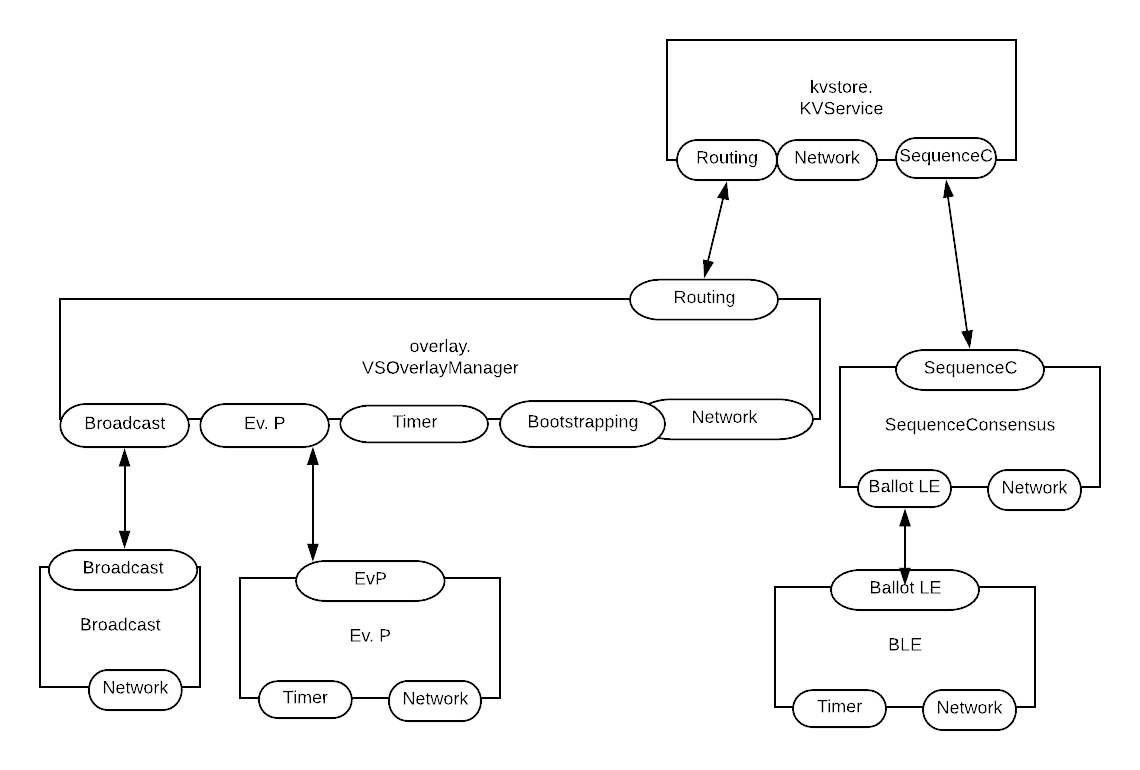
\includegraphics[scale=0.4]{Modified.png}
    \caption{Purview of the added components}
    \label{fig:modified}
  \end{center}
\end{figure}

The components from the exercises where copied for the most part, but refined in some ways to fit the use case.
Especially regarding the starting of _Ev.P_ and _BLE_ since the nodes don't know the other nodes in their replication group until bootstrapping is finished.


%Testing
\section{Testing}


%Respon
\section{Responsibilities}


%Conclusion
\section{Conclusion}


\end{document}
